\begin{figure}[htb!]
  \centering
  \begin{subfigure}[b]{0.35\textwidth}
    \centering
    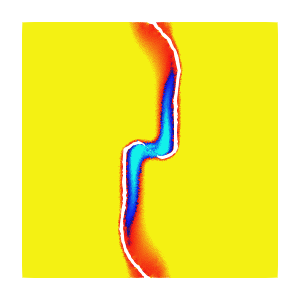
\includegraphics[width=\textwidth]{Chapter4/figures/biaxial_nosplit_stress.png}
  \end{subfigure}
  \begin{subfigure}[b]{0.15\textwidth}
    \centering
    \caption*{$\xnormal \cdot \stress \cdot \xnormal (\SI{}{\mega\pascal})$}
    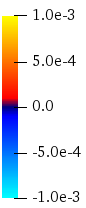
\includegraphics[width=0.7\textwidth]{Chapter4/figures/coldhot_pressure.png}
    \vspace{0.1in}
  \end{subfigure}
  \caption{Contour plot of the normal pressure right before the bridge forms. The pressure is calculated for an orientation that is estimated to be orthogonal to the bridge. Elements within the contour of $d = 0.75$ are removed to indicate the current crack set. }
  \label{fig: Chapter4/biaxial_nosplit_stress}
\end{figure}
